% Authors: Axel Wachtler, Joerg Wunsch, Matthias Vorwerk
% http://www.uracoli.de

\documentclass{beamer}
\usepackage{beamerthemeshadow}
\usepackage[ngerman]{babel}
\usepackage[utf8x]{inputenc}
\usepackage{graphicx}

\definecolor{slidyblue}{HTML}{527bbd} % lightblue headings from slidy

\newcommand{\Head}[1]{{\textbf{\textcolor{slidyblue}{#1}}}}

% \usetheme{Boadilla}

% \setbeamercovered{transparent}
% \beamertemplatenavigationsymbolsempty
\setbeamertemplate{footline}[frame number]
\setbeamertemplate{headline}{}

\title{Tic-Tac-Toe Reloaded}
\author{Jörg Wunsch, Axel Wachtler, Matthias Vorwerk}

\begin{document}

% \frame{\frametitle{Intro}
% \begin{figure}
% 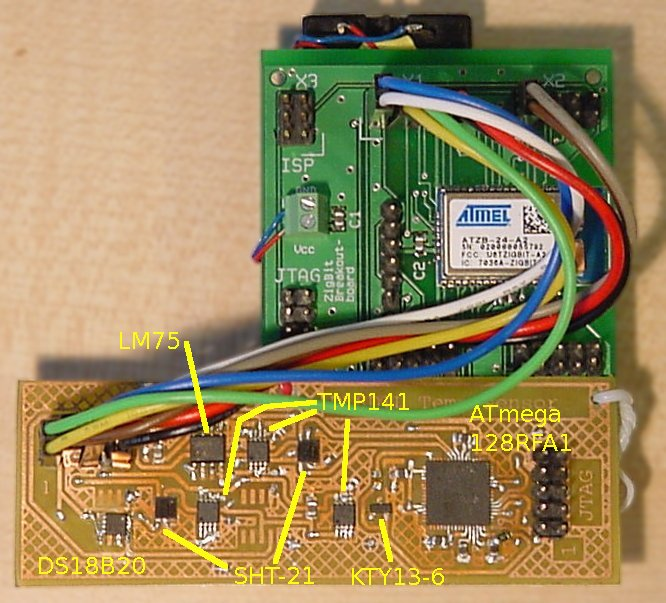
\includegraphics{../sensorboard.jpg}
% \caption{show an example picture}
% \end{figure}}

\frame{\titlepage}

% ----------------------------------------

\section{Einleitung}

\frame{\frametitle{Gliederung}
\tableofcontents
}

% ----------------------------------------

\section{Teil I - Die Hardware}

\frame{\frametitle{Die Platinen}
}

\frame{\frametitle{AVR Dragon anschließen}
}

% ----------------------------------------

\section{Teil II - ''Hallo Welt'' auf dem Mikrocontroller}

\frame{\frametitle{Programme für den AVR compilieren}
}

\frame{\frametitle{Programme auf den AVR laden}
}

\frame{\frametitle{Programme auf dem AVR debuggen}
}

% ----------------------------------------

\section{Teil III - Die LED und Touch Treiber}

\frame{\frametitle{Ansteuerung der LED-Matrix}
}


\frame{\frametitle{Abfrage der kapazitiven Touchpads}
}

\frame{\frametitle{Abfrage der resistiven Touchpads}
}

% ----------------------------------------

\section{Teil IV - Implementierung des Spiels}

\frame{\frametitle{Funkkomunikation}
}

\frame{\frametitle{Daten Senden}
}

\frame{\frametitle{Daten Empfangen}
}

\frame{\frametitle{Die Spiel Zustände}
}

\frame{\frametitle{Die Ergebnis-Auswertung}
}

% ----------------------------------------

\section{Teil V - Weitere Optimierungen}

\frame{\frametitle{Strom sparen}
}

% ----------------------------------------

\section{Danksagung}
\begin{frame}
\frametitle{Danksagung}

Wir möchten uns bei den folgenden Firmen und Personen
für die Unterstützung bei diesem Vortrag bedanken.

\vspace{0.3 cm}

\textbf{Atmel Germany GmbH}
für die Bereitstellung der Mikrocontroller vom Typ
ATmega128RFA1
\vspace{0.3 cm}

%\begin{figure}
%
\includegraphics[width=0.6\textwidth]{../sensirion_logo.jpg}
%\end{figure}
\texttt{http://www.atmel.com}

\vspace{0.3 cm}

\textbf{Platinensammler}
für die vergünstigte Leiterplattenherstellung.
\vspace{0.3 cm}

\end{frame}

% ----------------------------------------
\begin{frame}
\frametitle{Referenzen}

\begin{itemize}
\item \texttt{http://uracoli.nongnu.org/clt2012}
	\begin{itemize}
	\item Webseite zum Workshop
	\item Links zu weiteren Quellen
	\end{itemize}

\item \texttt{http://uracoli.nongnu.org}
	\begin{itemize}
	\item Projektwebseite
	\end{itemize}

\item {\small\texttt{http://lists.nongnu.org/mailman/listinfo/uracoli-devel}}%
	\begin{itemize}
	\item Entwickler Mailingliste
	\end{itemize}
\end{itemize}

\end{frame}

% TOC page (can be jumped to from PDF menu)

\begin{frame}
\tableofcontents
\end{frame}

\end{document}
